\documentclass{book}\usepackage{knitr}

% Preamble

%%%%%%%%%%%%%%%%%%%%%%
%% PACKAGES
%%%%%%%%%%%%%%%%%%%%%%
\usepackage[twoside,letterpaper,width=6in,height=8in]{geometry}
\usepackage{siunitx} % format units properly
\usepackage{wrapfig}
\usepackage[margin=10pt,font=small,labelfont=bf]{caption} % format captions
\usepackage{booktabs} % nicer tables
\usepackage{subcaption} 
\usepackage{csquotes} % block quotes
\usepackage{tikz}
\usepackage[inline, shortlabels]{enumitem} % inline enumeration
%\usepackage[version=4]{mhchem}
\usepackage{graphicx} % packages are used to modify the text and create bling.
%\includegraphics{{Home/CAMPUS/mwl04747/github/Environmnental-Sciences-in-East-Asia/images/}}
\usepackage{textcomp}
\usepackage{gensymb}
\usepackage{natbib}
\usepackage{glossaries}
\usepackage{amsmath}%
\usepackage{amsfonts}%
\usepackage{amssymb}%

%\usepackage[super,square,comma]{natbib}
%\usepackage{float}
%\usepackage{appendix}
%\usepackage{chngcntr}
%\usepackage{etoolbox}
%\usepackage[usenames]{xcolor}% for commenting in color!

\RequirePackage{hyperref} % For hyperlinked cross-references
\hypersetup{
    colorlinks,
    citecolor=blue,
    filecolor=blue,
    linkcolor=blue,
    urlcolor=blue
}


%----------------------------------------------------------
\newtheorem{theorem}{Theorem}
\newtheorem{acknowledgement}[theorem]{Acknowledgement}
\newtheorem{definition}[theorem]{Definition}
\newtheorem{example}[theorem]{Example}
\newtheorem{exercise}[theorem]{Exercise}

\newtheorem{problem}[theorem]{Problem}
\newtheorem{remark}[theorem]{Remark}
\newtheorem{solution}[theorem]{Solution}
\newtheorem{summary}[theorem]{Summary}
\newenvironment{proof}[1][Proof]{\textbf{#1.} }{\ \rule{0.5em}{0.5em}}
%----------------------------------------------------------

\AtBeginEnvironment{subappendices}{%
\chapter*{Appendix}
\addcontentsline{toc}{chapter}{Appendices}
%\counterwithin{figure}{section}
%\counterwithin{table}{section}
}

\makeatletter
\newcommand{\chapterauthor}[1]{%
  {\parindent0pt\vspace*{-25pt}%
  \linespread{1.1}\large\scshape#1%
  \par\nobreak\vspace*{35pt}}
  \@afterheading%
}
\makeatother

\renewcommand{\glstextformat}[1]{\textbf{\color{blue}\em #1}}

\newcommand{\R}{\mathbb{R}}
\newcommand{\carbondioxide}{CO$_2$~}



\title{Environmental Issues in East Asia}
\author{EA30e Spring 2021}
\date{\today}
\IfFileExists{upquote.sty}{\usepackage{upquote}}{}
\begin{document}

\maketitle
\makeglossaries

\frontmatter
\tableofcontents


\chapter*{Preface}

\section{Guiding Principles}

Environmental issues in East Asia are not unique or particularly more prevasive than other parts of the world. However, the issues are born from particular histories that may contrast with other parts of the world and other parts of the world may be able to learn from. 

In this project, the students in EA030e (Spring 2021) have written a textbook that highlights examples of environmental processes. Each student contributed to one theme, composed of two examples that highlight environmental issues of East Asia. 

\subsection{Context and Positionality}

As students in a college course located in Southern California, we approach the project with...


Our goal is not to call out environmental issues in East Asia, but to point to linkages of how a range of globalized economy contribute to these environmental problems. 

In the end, it would be useful for us to acknowledge we have some capacity to address these how these global linkages could be modified to reduce these environmental issues.

We are not experts, but learning... if there are errors please let us know... We recommend that suggestions be submitted via a github pull request.

\subsection{Goals}

Processes across horizontal boundaries define many environmental patterns that frame human interactions with the environment. How do humans impact processes that cross these boundaries and how do humans influence these ecosystem interface?

\subsection{Rationale}

We hope to learn more about the how environmental issues are expressed in different parts of the world and to what extent can we learn from this work. 

\subsection{Activity}

Each group will be composed of two students, that will become experts and teach their classmates on the topic. 

\section{East Asia and the World}







\section{Acknowledgments}

Everyone in the world!




\chapter{Author Guide}\label{ch:guide}

\subsection*{Why Learn \LaTeX?}

In the past, I used \LaTeX to make publication quality text. In fact, many prefer writing in \LaTeX because they can focus on the text and avoid worrying about formatting. However, it is NOT WYSIWYG (``what you see is what you get'') word processor. In reality, the processing or compiling is a separate step. 

Nevertheless, the quality of the output and ability to integrate with R (or Python) allows us to have an exceptional tool to make reproducible documents. 

\subsection*{How to Learn \LaTeX?}

There are several ways to learn \LaTeX. I suggest you find a decent tutorial to get the basics. For example, here are some suggestions:

\begin{itemize}
  \item \href{https://www.overleaf.com/learn/latex/Learn_LaTeX_in_30_minutes}{Learning \LaTeX in 30 minutes}
\end{itemize}

If you are like me and can't remember commands very well, then here's a \href{https://wch.github.io/latexsheet/latexsheet-0.png}{cheet sheet} that might be helpful. 

\subsubsection{R Chunks}

To create effective graphics, each chapter will have a rchunk that creates a graphic for the chapter. To review and learn R, here are some resources: 

\begin{itemize}
  \item \href{www.tbd.com}{Marc's Video Description}
  \item \href{https://rmd4sci.njtierney.com/}{RMarkdown for Scientists (super helpful!)}
  \item \href{https://rmarkdown.rstudio.com/lesson-1.html}{R Studio Tutorial}
  \item \href{https://rstudio.com/wp-content/uploads/2016/03/rmarkdown-cheatsheet-2.0.pdf?_ga=2.107420162.161662097.1613074083-214354297.1613074083}{R Studio's Cheatsheet}
  \item \href{https://bookdown.org/yihui/rmarkdown-cookbook}{R Markdown Cookbook -- Robust Source}
\end{itemize}


\subsection*{Noting Your Contribution}

Because this is an ongoing project, you should record your contribution to each chapter -- but also let go of these contributions at some point; Others might revise and their authorship might take some precedence, so you should both invest in the product but also be willing to detach from the final outcome as others contribute. This will feel uncomfortable at times, but please note from the beginning this is a social process and as such subject to negotiation. Please be generous to the authors that laid the foundation and be respectful of those that follow. 

\section{Setting Up Book Project--Type Setting w/ \LaTeX}

\subsection*{Latex Book Class}

Currently, the text is written using the standard book class. %However, in 2019, I (Los Huertos) will convert the format to a Tufte book class. 

\subsection*{Structuring the Text with Nested Hierarchies}

Contributors divide their contributions into sections and subsections. This format allows a consistent approach to structuring the text and forcing themes to be organized in blocks that can be used to organize the overall text. We use section, subsection, and subsubsection to break up the topic into bite sizes. 

To accomplish this, contributors use the \verb"\section{Section}" command for major sections, and the \verb"\subsection{Subsection}" command for subsections, and a similar approach for subsubsections. 

NOTE: for each nested level, it MUST be followed by the lowest level in the section before a paragraph is started -- in contrast to what is shown above!

NOTE: We may dispense with subsubsections in the future to provide a less blocky structure, but for now they remain useful. 

\subsection*{Font Changes}

We can use various methods to alter the typeset: \emph{Emphasize}, \textbf{Bold}, \textit{Italics}, and \textsl{Slanted}. We can also typeset \textrm{Roman}, \textsf{Sans Serif}, \textsc{Small Caps}, and \texttt{Typewriter} texts.  Look online to see the commands to accomplish these changes. 

You can also apply the special, mathematics only commands $\mathbb{BLACKBOARD}$, $\mathbb{BOLD}$, $\mathcal{CALLIGRAPHIC}$, and $\mathfrak{fraktur}$. Note that blackboard bold and calligraphic are correct only when applied to uppercase letters A through Z.

You can apply the size tags -- Format menu, Font size submenu -- {\tiny tiny}, {\scriptsize scriptsize}, {\footnotesize footnotesize}, {\small small}, {\normalsize normalsize}, {\large large}, {\Large Large}, {\LARGE LARGE}, {\huge huge} and {\Huge Huge}.

You can use the \verb"\begin{quote} etc. \end{quote}" environment for typesetting short quotations. Select the text then click on Insert, Quotations, Short Quotations:

\begin{quote}
The buck stops here. \emph{Harry Truman}

Ask not what your country can do for you; ask what you can do for your
country. \emph{John F Kennedy}

I am not a crook. \emph{Richard Nixon}

I did not have sexual relations with that woman, Miss Lewinsky. \emph{Bill Clinton}
\end{quote}

The Quotation environment is used for quotations of more than one paragraph. Following is the beginning of description of \LaTeX from \emph{Wikipedia}:

\begin{quotation}
LaTeX (/ˈlɑːtɛx/ LAH-tekh or /ˈleɪtɛx/ LAY-tekh, often stylized as \LaTeX) is a software system for document preparation. When writing, the writer uses plain text as opposed to the formatted text found in ``What You See Is What You Get'' word processors like Microsoft Word, LibreOffice Writer and Apple Pages. The writer uses markup tagging conventions to define the general structure of a document (such as article, book, and letter), to stylise text throughout a document (such as bold and italics), and to add citations and cross-references. A \TeX distribution such as \TeX Live or MiK\TeX is used to produce an output file (such as PDF or DVI) suitable for printing or digital distribution.

LaTeX is widely used in academia for the communication and publication of scientific documents in many fields, including mathematics, statistics, computer science, engineering, physics, economics, linguistics, quantitative psychology, philosophy, and political science. It also has a prominent role in the preparation and publication of books and articles that contain complex multilingual materials, such as Sanskrit and Greek. \LaTeX uses the TeX typesetting program for formatting its output, and is itself written in the TeX macro language.''
\end{quotation}

Use the Verbatim environment if you want \LaTeX\ to preserve spacing, perhaps when
including a fragment from a program such as:
\begin{verbatim}
#include <iostream>         // < > is used for standard libraries.
void main(void)             // ''main'' method always called first.
{
 cout << ''This is a message.'';
                            // Send to output stream.
}
\end{verbatim}
(After selecting the text click on Insert, Code Environments, Code.)


\subsection*{Mathematics and Text}

\subsubsection{Warning: Special Characters}

When you use percent and ampersand symbols, hash tags, and other non-standard ASCII characters, \LaTeX will be very uncooperative. So, do yourself a favor and make sure you understand that these are used for special typesetting functions. To use them you have to ``escape'' and use commands to get them to do what you might usually expect!  \% \# \& \`e \~n `` and '' to show a few that do not reflect the key stroke you might expect. 

\LaTeX doesn't like a range of characters or they reserved for special behavior...

For example, the \# is used for tabs in a table environment. \% is used to make comments, thus stuff behind a \% is ignored. There are lots of others, but these come up the most.

\subsubsection{Creating equations}

One of the most powerful parts of \LaTeX is how it can be used to write complex equations, with all those symbols and Greek letters! This can be done inline $y = mx + b + \epsilon$ for fairly simple equations, or set apart for more complex equations:

\begin{equation}
\int_0^\infty e^{-x^2} dx=\frac{\sqrt{\pi}}{2}
\end{equation}

\subsubsection{Theorems, etc}
\begin{theorem}
(The Currant minimax principle.) Let $T$ be completely continuous selfadjoint operator
in a Hilbert space $H$. Let $n$ be an arbitrary integer and let $u_1,\ldots,u_{n-1}$ be
an arbitrary system of $n-1$ linearly independent elements of $H$. Denote
\begin{equation}
\max_{\substack{v\in H, v\neq
0\\(v,u_1)=0,\ldots,(v,u_n)=0}}\frac{(Tv,v)}{(v,v)}=m(u_1,\ldots, u_{n-1})
\label{eqn10}
\end{equation}
Then the $n$-th eigenvalue of $T$ is equal to the minimum of these maxima, when
minimizing over all linearly independent systems $u_1,\ldots u_{n-1}$ in $H$,
\begin{equation}
\mu_n = \min_{\substack{u_1,\ldots, u_{n-1}\in H}} m(u_1,\ldots, u_{n-1}) \label{eqn20}
\end{equation}
\end{theorem}
The above equations are automatically numbered as equation (\ref{eqn10}) and
(\ref{eqn20}).


\subsection{Lists Environments: Making bulletted, numbered, description lists}

We use special commands to create an itemized list.

You can create numbered, bulleted, and description lists
(Use the Itemization or Enumeration buttons, or click on the Insert menu
then chose an item from the Enumeration submenu):

\begin{enumerate}
\item List item 1

\item List item 2

\begin{enumerate}
\item A list item under a list item.

\item Just another list item under a list item.

\begin{enumerate}
\item Third level list item under a list item.

\begin{enumerate}
\item Fourth and final level of list items allowed.
\end{enumerate}
\end{enumerate}
\end{enumerate}
\end{enumerate}

\begin{itemize}
\item Bullet item 1

\item Bullet item 2

\begin{itemize}
\item Second level bullet item.

\begin{itemize}
\item Third level bullet item.

\begin{itemize}
\item Fourth (and final) level bullet item.
\end{itemize}
\end{itemize}
\end{itemize}
\end{itemize}

\begin{description}
\item[Description List] Each description list item has a term followed by the
description of that term.

\item[Bunyip] Mythical beast of Australian Aboriginal legends.
\end{description}

\subsection{Theorem-Like Environments}

The following theorem-like environments (in alphabetical order) are available
in this style.

%\begin{acknowledgement}
%This is an acknowledgement
%\end{acknowledgement}

\begin{example}
This is an example
\end{example}

\begin{exercise}
This is an exercise
\end{exercise}


%\begin{proof}
%This is the proof of the lemma.
%\end{proof}

%\begin{notation}
%This is notation
%\end{notation}

%\begin{problem}
%This is a problem
%\end{problem}

%\begin{proposition}
%This is a proposition
%\end{proposition}

%\begin{remark}
%This is a remark
%\end{remark}

%\begin{summary}
%This is a summary
%\end{summary}

\begin{theorem}
This is a theorem
\end{theorem}

%\begin{proof}
%[Proof of the Main Theorem]This is the proof.
%\end{proof}

%\subsubsection{``Child'' Rnw Contributions}

%This is a chapter that we can input into the text... you will each create a chapter without the preamble and begin and end document... that can be integrated into a single book! 

\subsection{Peer Review Commenting}

You can put your comments in square brackets and in color for things that need help. \textcolor{red}{[This section is confusing, I am not sure what commenting means.]}

\subsection{Adding Figures, etc}

\subsubsection{Using Rnw Files}

To generate R figures, we use R chunks in and Rnw file, where the text is integreated. When we compile into a PDF, the program converts the files into TeX files and then combineds them into a single pdf. 

For each chapter, we create a ``child'' document and Marc will help you create that text when you begin. 

\subsubsection{Creating a floating figure}

This is my floating figure (Figure \ref{fig:plot}).

\begin{figure}

\caption{My plot's caption is here!}
\label{fig:plot}
\end{figure}

\subsubsection{Using R to Create Effective Figures}

R Markdown can be a very powerful tool to integrate R code, figures and text. Making high quality figures that are both clear and aestically pleasing will be something that we need to think about it. 

\begin{itemize}
  \item Axis Labels -- Labelled with clarity 
  \item Axis Text -- Size, Orientation 
  \item Captions (usually better than titles)
  \item References connecting labels to references
  \item ADA accessible (e.g. color impairment mitigation)
\end{itemize}

For example, here's code to generate a pretty good figure: 



\begin{knitrout}
\definecolor{shadecolor}{rgb}{0.969, 0.969, 0.969}\color{fgcolor}\begin{kframe}


{\ttfamily\noindent\bfseries\color{errorcolor}{\#\# Error in file(file, "{}rt"{}): cannot open the connection}}

{\ttfamily\noindent\bfseries\color{errorcolor}{\#\# Error in createDataPartition(., p = 0.8, list = FALSE): object 'maunaloa' not found}}

{\ttfamily\noindent\bfseries\color{errorcolor}{\#\# Error in eval(expr, envir, enclos): object 'maunaloa' not found}}

{\ttfamily\noindent\bfseries\color{errorcolor}{\#\# Error in eval(expr, envir, enclos): object 'maunaloa' not found}}

{\ttfamily\noindent\bfseries\color{errorcolor}{\#\# Error in eval(expr, envir, enclos): object 'maunaloa' not found}}

{\ttfamily\noindent\bfseries\color{errorcolor}{\#\# Error in is.data.frame(data): object 'maunaloa' not found}}

{\ttfamily\noindent\bfseries\color{errorcolor}{\#\# Error in summary(model): object 'model' not found}}

{\ttfamily\noindent\bfseries\color{errorcolor}{\#\# Error in predict(., test.data): object 'model' not found}}

{\ttfamily\noindent\bfseries\color{errorcolor}{\#\# Error in mean((pred - obs)\textasciicircum{}2, na.rm = na.rm): object 'predictions' not found}}\end{kframe}
\end{knitrout}

In the case of Figure \ref(fig:maunaloa), we can a create a figure that has all of the characteristics listed above, except perhaps ADA. Creating a "alt text" for the figure is something we might want to consider. 

\begin{figure}
\begin{knitrout}
\definecolor{shadecolor}{rgb}{0.969, 0.969, 0.969}\color{fgcolor}\begin{kframe}


{\ttfamily\noindent\bfseries\color{errorcolor}{\#\# Error in ggplot(train.data, aes(decimal.date, average)): object 'train.data' not found}}\end{kframe}
\end{knitrout}
\caption{Carbon Dioxide Concentrations (Mauna Loa, HI). Source: Scripps/NOAA.}
\label{fig:co2-graphic}
\end{figure}

\subsection{Using Boxes}

\fbox{
\begin{minipage}[c]{.9\textwidth}
\subsection{minibox X}

Some text
\end{minipage}
}

\subsection{ Cross-References, Citations, and Glossaries}

\subsubsection{Cross-References}

We can cross-reference sections (e.g. Section~\ref{ch:critical-zone}  or figures (Figure~\ref{fig:maunaloa}) using several methods. I suggest you look at the this Rmd file to see how I did it in these examples.

You can also create links to URLs or hyperlinks, e.g. \url{http://texblog.org}. However, if these addresses change, then the link will break, so I suggest you only link to internal references.

\subsubsection{Bibliography generation}

There will be two steps to cite our sources. First, we need to add the reference to a database, or bib file. This is titled 'References.bib' and is located in the main folder in our respository. When you add information to the bib file, be sure to paste in the reference using a bibTeX format. 

Second, we'll need to place in-line citations, using \verb"\citep{knitr}", which produces \citep{knitr}, by using a key, which is knitr in this case. 

For example, you might write, ``This document was produced in RStudio using the knitr package (\citep{knitr}). Also try \verb"\citet{LosHuertos2017OverviewR}" to create use the author name as the subject: \citet{LosHuertos2017OverviewR} wrote an guide to help students learn R. 

Note: You will see these citations automatically put in alphabetic order in the Bibliography at the end of the PDF. 

%Currently, we are using the ecology.bst, but it has trouble with misc type of references, so I will changing this in 2019. 

\subsubsection{Creating glossary words}
 
\newglossaryentry{peat}{
	name=peat, 
	description={is cool.}
}

\begin{definition}
This is a definition and the word is use in an glossary, e.g. \gls{peat}. \Gls{peat} is when you want to capitalize the defined word without having to re-define a capitalized version, the only downside of case sensitivity in \LaTeX.
\end{definition}


\chapter{Chapter Title}

\chapterauthor{Chapter Author Name}

\footnote{Statement of Contributions-- For example, ``The chapter was first drafted by Marc Los Huertos (2021). The author recieved valuable feedback from X, and Y and Z to improve the chapter. Slater revised the chapter in 2022 with suggestions from Cater.'' Note: I am still working on the formatting for this to improve it.}

\section{Section Heading}% Avoid putting text between section and subsection headings.

\subsection{Subsection Headings} % Avoid putting text between subsection and subsubsection headings. Not applicable if you don't have subsections!

Some text here... if you cut and paste, be sure to make sure you don't include formatted characters outside the ASCII values. See Author Guide\ref{ch:guide}.

\subsubsection{Optional Subsubsection Headings} % Again try to avoid putting text between the subheadig and the subsubheading to main a structural consistency.

some text here....

\section{Goals of this template}

This template will NOT teach you how to use \LaTeX! To accomplish that, we'll rely on some great online resources that you can find on in Chapter \ref{ch:guide}. 

Instead this section of the document is designed to demonstrate how our textbook will look, feel, and ultimately how we contribute to the project.

This document also compiles all of our projects into a single PDF, where each chapter is composed of a input tex file.

\section{Here's figure}

\subsection{R Created Figures}

First we create an R chunk and add some code. In this case, I created a floating figure which can be referenced (Figure~\ref{fig:pressure})!  

\begin{figure}
\begin{knitrout}
\definecolor{shadecolor}{rgb}{0.969, 0.969, 0.969}\color{fgcolor}\begin{kframe}
\begin{alltt}
\hlkwd{plot}\hlstd{(pressure)}
\end{alltt}
\end{kframe}
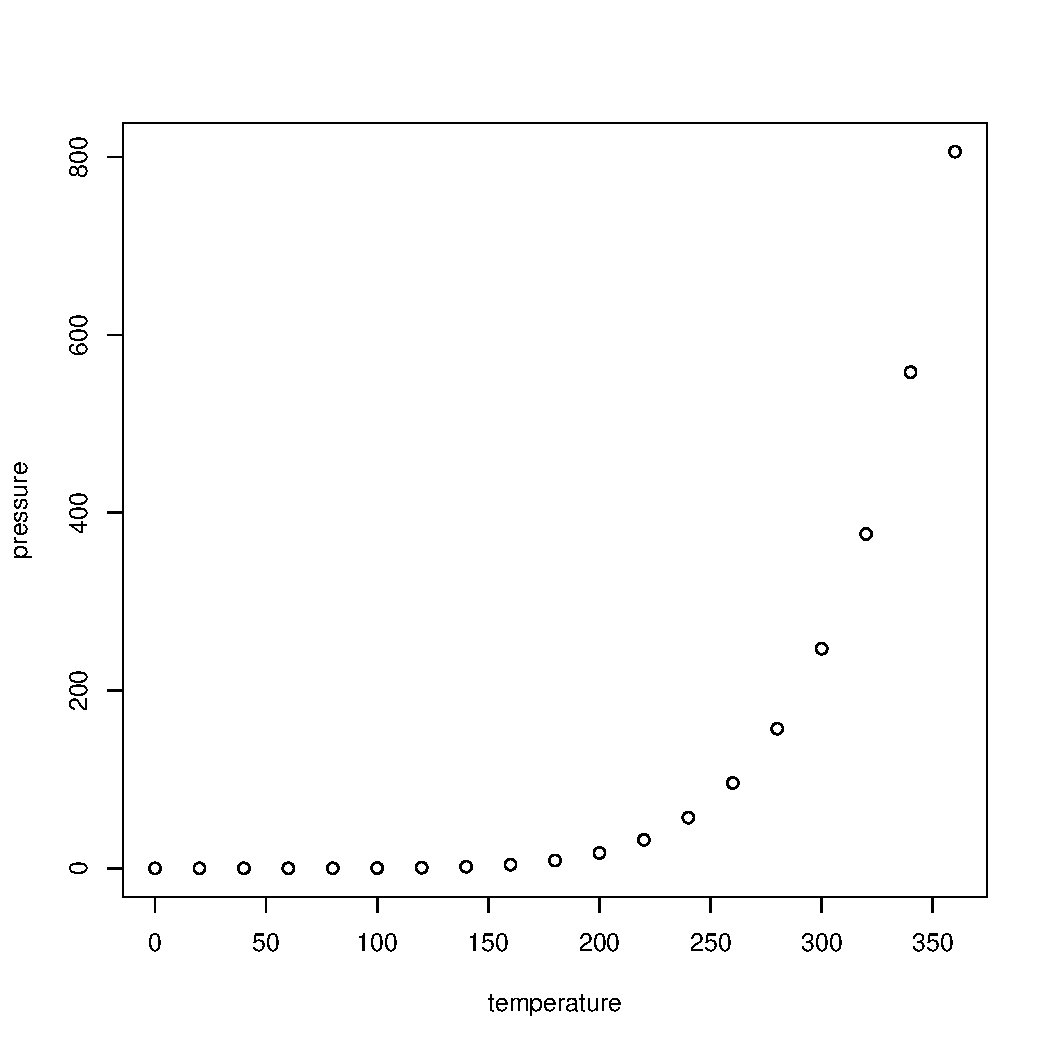
\includegraphics[width=\maxwidth]{figure/fig:pressure-1} 

\end{knitrout}
\caption{Figure Caption...we should turn "echo=False" in the R chunk options, but I left it true for now. (source: ??)} % define the caption, then the label.
\label{fig:pressure}

\end{figure}

\subsection{Floating Figures from External Sources}

All figures and images that are imported should be put into the "images" sudirectory to keep stuff organized. Even better to create a subdirectory with your images, but we can naviagate as we go.

Figure \ref{fig:vadose} is a good example of inserting an image from an external source.

\begin{figure}
\includegraphics[width=\linewidth]{images/Lee-Vadose}
\caption{Vadose zone is neato (Source: \citet{lee2017fifty}).}
\label{fig:vadose}
\end{figure}

In this case, I had to specify the width so it would fit on the page!  See the Rnw file for the code. Notice, I was also abel to ``reference'' the figure in the text.

\section{Adding Citations}

See the Guide, as well, but my video is probably the most helpful.


Generally, there are many environmental trends in Asia \citep{imura2005urban}.

\citet{imura2005urban} describes the how urbanization has affected the hydrology of East Asia. 
 

\chapter{Title...}

\chapterauthor{Nora}

$\rightarrow$

\section{What the Polar Vortex and why do we care?}

\subsection{What Factors Drive Land Use Change?}





\mainmatter


\chapter{The Earth System}\label{earthsystem}

\chapterauthor{Marc Los Huertos}

\section{The Sun's Energy and the Earth's Temperature}

The temperture of the Earth's surface is the result of a balance -- the energy entering the atmosphere and the leaving the atmosphere. Most of this energy is in the form of light or electromagnetic radiation (Figure~\ref{fig:earthbudget}). 

\begin{figure}
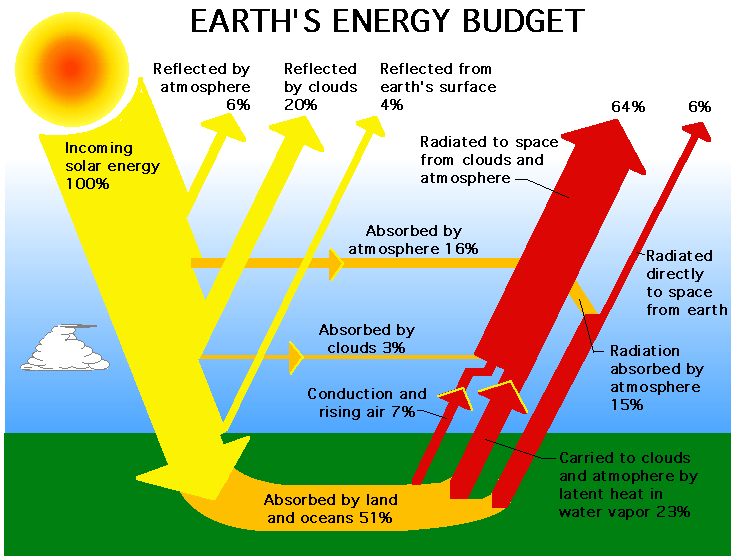
\includegraphics[width=\linewidth]{images/earth-system/earth-rad-budget-nasa-erbe.png}
\caption{caption}
\label{fig:earthbudget}
\end{figure}

Light enters the atmosphere, where some is absorbed and some is reflected. Light interacts in different ways with land, oceans, and vegetation, which is beyond the scope of our project. The ``quality'' of light changes through these processes. 

\subsection{The Spectrum of Light Entering and Exiting the Earth's Surface}

As the sun's electromagnetic radiation interacts with the Earth's Atmosphere, certain wavelengths are absorbed and filtered out (Figure~ \ref{fig:em-entering}).

\begin{figure}
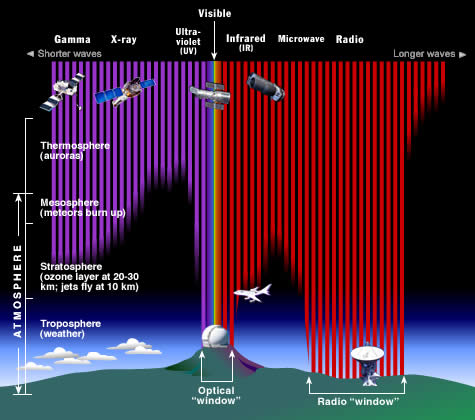
\includegraphics[width=\linewidth]{images/earth-system/em-radiation-atmosph-depth-stsci.jpg}
\caption{Various wavelengths of solar electromagnetic radiation penetrate Earth's atmosphere to various depths. Fortunately for us, all of the high energy X-rays and most UV is filtered out long before it reaches the ground. Much of the infrared radiation is also absorbed by our atmosphere far above our heads. Most radio waves do make it to the ground, along with a narrow `window' of IR, UV, and visible light frequencies. Source: STCI/JHU/NASA.}
\label{fig:em-entering}
\end{figure}

\subsection{The Atmosphere and Greenhouse Effect}



\section{Carbon Biogeochemistry}

\subsection{Long and Short Time Scales}

The carbon cycle processes occur at wide range of temporal scales from hundreds of millions of years to seasons of the year. These have been referred to as long and short carbon cycles. However, for our purposes, I will call them ``geologic carbon'' and ''biosphere carbon'' processes. 

\subsection{Rock Cycle and Geologic Carbon}

The carbon cycle describes changes in the fluxes and reservoirs of carbon in the Earth system. On very long time-scales, millions of years, the primary reservoirs of carbon are the atmosphere, ocean, and rocks (limestone). Carbon moves between these reservoirs through volcanic outgassing, silicate weathering, and limestone sedimentation. The carbon cycle is linked to Earth's energy balance through atmospheric carbon in the form of \carbondioxide, a greenhouse gas.

\subsubsection{Mountains and Erosion}

\ref{fig:carbonpools}

\begin{figure}
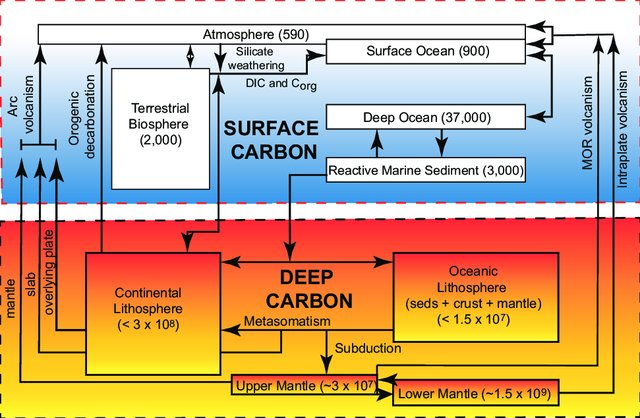
\includegraphics[width=\linewidth]{images/earth-system/Carbon-reservoirs-and-cycles-in-the-Earth.jpg}
\caption{Carbon reservoirs and cycles in the Earth. The figure shows short-and long-term cycles; biosphere and geologic carbon reservoirs and fluxes, and the relative sizes and residence times (y axis) of respective carbon. Numbers in brackets refer to the total mass of carbon in a given reservoir, in Pg C (1Pg C = 10$^{15}$ g carbon). All reservoirs are pre-industrial. Abbreviations: C org = organic carbon; DIC = dissolved inorganic carbon; MOR = mid ocean ridge; seds = sedimentary rocks. Adapted from Lee et al. (2019 And references therein).}
\label{fig:carbonpools}
\end{figure}

\subsubsection{Subduction Burial and Carbon Recycling}

Figure~\ref{fig:longtermcarbon}

\begin{figure}
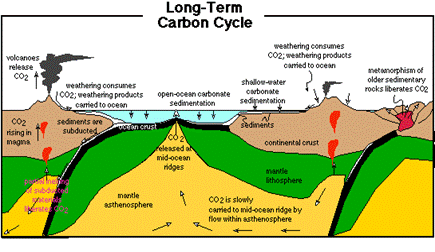
\includegraphics[width=\linewidth]{images/earth-system/long-term-carbon.png}
\caption{Schematic of the long-term carbon cycle (from Bice, 2001)}
\label{longtermcarbon}
\end{figure}

\subsection{Photosynthesis, Respiration, and Biosphere Carbon}

\subsubsection{Soil Respiration and the Soil Profile}

Carbon in soils is respired -- but different pools might have different rates of respiration. Sometimes these pools are distinquished as an active soil organic carbon pool and slow soil organic carbon pool. Although the reference of ``slow'' causes confusion with long-term, geologic carbon, but soil organic carbon remains a component of what we are refering to as biosphere carbon. 

The surface of the soil tends to have more SOC and microbes that can use that carbon for respiration. Lower down in the soil profile, we tend to see lower amounts of SOC and lower microbial biomass (Figure~\ref{fig:soilcarbon}. In addition, soils in the lower part of the profile tend to have more aggregation that protects SOC from microbial attack, thus a key area that soil carbon can seqeustor carbon. 

In addition to these microbial biomass and aggregate patterns, the microbes aree more senstive to temperature changes near the surface as measured by Q10 -- the rate of biochemical processes with a 10 degree C increase in temperature. Thus, soil processes, such as respiration, is likely to increase more near the surface with global warming that the lower part of the soil profile.  

\begin{figure}
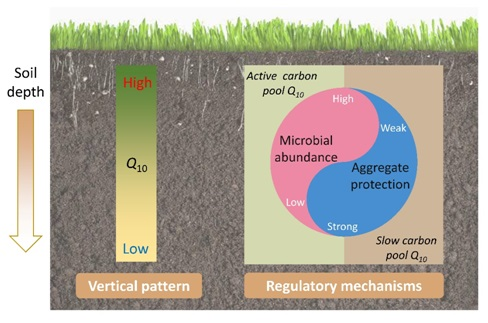
\includegraphics[width=\linewidth]{images/earth-system/Q10-SOC-Regulation.jpg}
\caption{Regulatory Mechanisms of the Temperature Sensitivity of Soil Organic Matter Decomposition in Alpine Grasslands (Source: \citet{Qineaau1218, CAS2021researchers}).}
\label{fig:Q10-SOC}
\end{figure}


\section{Fossil Fuels and Carbon Dioxide Trends}\label{sec:fossilfuels}

As part if the industrial revolution, our energy sources have put more \carbondioxide from the biosphere (soils and forests) and geologic carbon (coal, petroleum). 

\subsection{The Signal of Geologic and Biosphere Carbon in Atmosphere}

The combined contribution from geologic and biosphere carbon in the atmosphere is clearly documented from numerous sources. First, look at data collected at the Mauna Loa where \carbondioxide measurements have been taken continuously since the late 1950s. 

Figure~\ref{fig:maunaloa2}

\begin{figure}
\begin{knitrout}
\definecolor{shadecolor}{rgb}{0.969, 0.969, 0.969}\color{fgcolor}\begin{kframe}


{\ttfamily\noindent\bfseries\color{errorcolor}{\#\# Error in ggplot(train.data, aes(decimal.date, average)): object 'train.data' not found}}\end{kframe}
\end{knitrout}
\caption{Carbon Dioxide Measure on Mauna Loa, HI}
\label{fig:maunaloa2}
\end{figure}






\chapter{Monsoons and East Asia Climates}

\section{Temperature Gradients and Latitude}





\chapter{Critical Zone}\label{ch:critical-zone}

\chapterauthor{Marc Los Huertos}\footnote{The chapter was first drafted by Marc Los Huertos (2021). The author recieved valuable feedback from X, and Y and Z to improve the chapter.}

\section{What is the Critical Zone}

The crticical zone refers the the portion of the Earth's skin where the zone where rock meets life. The Critical Zone supports all terrestrial life.

The critical zone includes the following:

\begin{itemize}
  \item A permeable layer from the tops of the trees to the bottom of the groundwater;
  \item An environment where rock, soil, water, air, and living organisms interact and shape the Earth's surface;
  \item Water and atmospheric gases move through the porous Critical Zone, and living systems thrive in its surface and subsurface environments, shaped over time by biota, geology, and climate.
\end{itemize}

All this activity transforms rock and biomass into the central component of the Critical Zone - soil; it also creates one of the most heterogenous and complex regions on Earth.

Its complex interactions regulate the natural habitat and determine the availability of life-sustaining resources, such as food production and water quality.

These are but two of the many benefits or services provided by the Critical Zone. Such `Critical-Zone Services' expand upon the benefits provided by ecosystems to also include the coupled hydrologic, geochemical, and geomorphic processes that underpin those ecosystems.

\begin{figure}
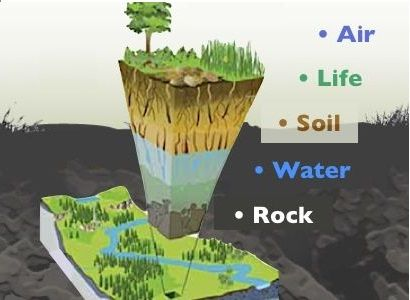
\includegraphics[width=\textwidth]{images/critical-zone/criticalzone.jpg}
\caption{The Critical Zone is an interdisciplinary field of research exploring the interactions among the land surface, vegetation, and water bodies, and extends through the pedosphere, unsaturated vadose zone, and saturated groundwater zone. Critical Zone science is the integration of Earth surface processes (such as landscape evolution, weathering, hydrology, geochemistry, and ecology) at multiple spatial and temporal scales and across anthropogenic gradients. These processes impact mass and energy exchange necessary for biomass productivity, chemical cycling, and water storage.}
\label{fig:criticalzone}
\end{figure}

\subsection{What are the environmental implications of the Critical Zone?}

The critical zone as a concept and as a material space pushes us to think of the porousity of the Earth's surface --- the gas and fluid flows through rocks, soils, and plants. We can begin to appreciate the complexity of the transport and fate of chemical pollutants as they enter the soil and become part of the vadose zone and perhaps the ground water table -- moving with water and diffusing through the water, simultaneously.

\section{Hydrologic Aspects}

\subsection{The Vadose Zone}

Jeji is a volcanic island is located some XX km south of the Korean Penisula. Water runs off the steep slopes quickly and water supplies are limited on the island. To adddress this...\citet{lee2017fifty}.

\begin{figure}
\includegraphics[width=\linewidth]{images/critical-zone/Lee-Vadose.png}
\caption{... (Source: \citep{lee2017fifty}).}
\label{fig:vadose2}
\end{figure}



\chapter{Land Use in East Asia}

chapterauthor{Samantha Beaton}

What is Land Use Change?

What Factors Drive Land Use Change?

How Land Use Change is Measured and Quantified

Integration of sociology

with data science: spatial data compiled from aerial photos, Landsat satellite images, topographic maps, GPS data, etc.

Requires classification and division of land-space types

Ecological Effects of Land Use Change on Soil, Air, and Water

\section{Impacts on Soil}

Deforestation and soil degradation

lack of stability (erosion) and loss of carbon sequestration potential

Forests


coupled with monoculture agriculture

Example Case Study: representative of monoculture agriculture-rice paddies in SE Asia (potentially\ldots)


Impacts on Local Watersheds

hydrology 

infiltration/pollution, groundwater recharge, flow of river basins, runoff

Higher risk of flooding and droughts

\section{Conclusion \& Prospect of Sustainable Urbanization/Land Use Change}


\chapter{Nuclear Power and Nuclear Waste}

\section{Current and Future Energy Needs}



\chapter{Air Pollution \& Social Justice in Hong Kong}

\chapterauthor{Neenah Vittum}

\section{Science of Air Pollution}

\subsection{Overview of the layers of the atmosphere/atmospheric gases}

What part of the atmosphere does air pollution affect?

What is air pollution?

Overview of different types of air pollution

\section{Major Sources → Use as geographical overview}

\subsection{General common sources of air pollution all over the world}

\subsection{East Asian countries/communities and their prominent air pollution sources}

Shipping

Traffic Emissions

Commercial and otherwise

Coal

Urban Development

Manufacturing

Other

The transboundary issue and its implications in regulation and politics

Impacts

Human health

Environmental Health

Greenhouse gas emissions and global warming

Both

Visibility

Environmental Justice

Case Study: Hong Kong

The Intersection of Air Pollution and Other Environmental Issues

Many environmental issues are interconnected

Air pollution and deforestation

Air pollution and urbanization/industrialization

Other Issues (To Explore)

Goals/Other Ideas/Questions

Ground information in geography and relevant examples

Incorporate stories and person accounts

slow violence → environmental justice issues

Maybe activist or someone who has suffered the issues firsthand

Draw people into the empathy

Use stories and descriptions to describe places

What is the best way to section the chapter?


\chapter{Flood Pulse System in East Asia}

\chapterauthor{Kristin Gabriel}

\section{Introduction}

What is the flood pulse system?

Seasonality

Ecosystem Services

Fish stocks

Flooded forests

How the flood pulse system influences the Tonle Sap Ecosystem

Timing of Flood Pulse

Magnitude of Flood Pulse

Duration of Flood Pulse

Influence of flood pulse system on people and their livelihoods

Fisheries

Immigration and emigration

Human Impacts on the flood pulse system

Climate change

Dam development

Case Study: Cambodia and the Tonle Sap


\chapter{Hydroelectric Dams in East Asia}

\section{Introduction}

Basic facts about dams in East Asia


Statistics on how many, size, scale, location etc.

Function of the Dam 

How it generates electricity/how much

Different types of dams (multi/single use etc.) 

Immediate ecological impacts 

Positive: 

Flood control, electricity generation, improved water quality 

Negative: 

Decreased water quality, flooding, sedimentation, habitat loss, deforestation, salinization etc... *note: the ecological impacts may be too many to go completely in depth into so perhaps a paragraph or subsection of each as opposed to a 7 page explanation of each 

Anthropological impacts 

Supposedly positive (I.e. employment etc...)

Negative: displacement, loss of cultural sites, diseases 

Displacement

Policy/government action/regulation  (policies that exist or propose solutions)

\section{Conclusion}



\chapter{Climate Change and Food Security in Myanmar}



\section{Climate Change, Climate Change Response in Myanmar}


General history of rice production and food demand in Myanmar. 

Impact on credit policy on rice 

Impact of infrastructure development on rice production

Study of the constraints of rice production in Myanmar

The effect of a command economy on food production in Myanmar 

Overall review on demand for food in Myanmar 

Possible implementation of SRI (systemic rice intensification) in order to increase rice yields in Myanmar

Transition from talking about rice production

sea-level rise

subsidence

coastal erosion

coastal flooding

Impact of climate change on rice production in Southeast Asia

Monsoon Season effect on Ayeyarwady River Badin

Sea Level Rise 

Sea level rise effect on global markets/rice production


Subsidence

Subsidence in Yangon, Myanmar

interview segments/personal experiences of rice farmers


Roles of the Burmese government

\section{Conclusion}

Reminders/Areas of Focus




\chapter{Disasters, Typhoons and Phillipines}

\chapterauthor{Ian Horsburgh}

\section{What are Typhoons?}



\chapter{Climate Infrastructure in Vietnam}

\section{Introductory}

How climate change will impact Vietnam

Flooding (especially coastal urban areas)

Sea Level Rise

Land Erosion

Health outcomes

Current Adaptation Plans

Strengthen existing barriers and infrastructure

Adapt cities expecting sea level rise

Withdraw from the coastlines in areas that are well below sea level

What's Needed for the Future

Stronger healthcare system

Support for farmers and agricultural workers

Support for rural population near Mekong and Red river deltas

\section{Conclusion}

Implications for other places in the region


\chapter{Wastewater Management for a Circular Economy}
\chapterauthor{Matias Ceccarelli}

\section{Overview}

The First Law of Thermodynamics states: ``energy can be neither created nor destroyed, but can be transformed from one form to another.'' The energy constituting Earth’s resources is constant but always changing form. By understanding this law we can begin to outline sustainable waste management systems and shift from a linear extraction based/single-use economy, to a regenerative circular economy that sustains human/environmental health. While every human activity generates waste, in nature, waste does not exist. Nature operates as a circular system, turning decay into energy; nature is the model for a circular economy; it inspires biomimetic systems that function as a whole in synergy with the environment.

The majority of the world uses a linear supply chain model, ending with disposal rather than reusal. Circularity is gaining enormous traction as the best way to sustain life on Earth. The United Nations and international governments are echoing the need to transition from a linear to a circular economy. Circularity is a way of life still practiced by first nation peoples around the world: ``do not take more than you need,'' ``replenish what is taken'' \citep{sharp_2019}. 

Waste management is an important yet often forgotten sector underlying all systems. It is the foundation of a circular economy. It’s not within this paper’s scope to cover the intricacies of the supply chain, waste management, or circular economics; covered here is an analysis of linear and circular wastewater treatment systems that process sustainable and unsustainable waste from household, industrial, and agricultural facilities. This paper agrees, linear-waste is unsustainable and a danger to humans and the environment \citep{mustafa2020recent} \citep{braungart_mcdonough_kroese_2011}  \citep{bown}. This paper postulates that if sustainable-waste is processed by bio-regenerative-wastewater-treatment-systems, defined by ingredient recovery apparatus, a circular economy will be more readily realized and humans as well as the environment will prosper. It is hoped this analysis will elucidate the interdependence of all systems, human and nonhuman, through life's fundamental element––water. This analysis is organized by multiple case studies examining distinct linear and circular wastewater treatment systems in SouthEast Asia. Here, linear wastewater treatment includes: open defecation, septic latrines, and the majority of municipal sewage waste treatment facilities; Linear waste includes pesticides and chemicals; Circular wastewater treatment includes: double-vault-compost latrines, anaerobic digesters with biogas recovery, and phytoremediation systems. Linear ends with waste; circular is wasteless. 

\subsection{Linear Economy}

The primary challenge of sustainable development comes from the energy/material stream between humans and the environment. The current and traditional linear production model: ``take, make, [use], waste,'' is unsustainable and originates from the Industrialization Revolution (1760-1840) \citep{braungart_mcdonough_kroese_2011}. The linear-supply-chain is fueled by the desire to make products as fast as possible, produce the greatest number of goods, and deliver them to the highest number of people. This process is often extractive and harmful to the environment (convenience economics). Standardized mass-production regards Earth's limited resources as endless; reuse is not a function, instead, disposal is the outcome. Pollutants generated are harmful to humans and the environment. The linear system is a major source of today’s socio-economic injustices; it is the source of climate change 
\citep{braungart_mcdonough_kroese_2011}. 

The linear system begins with raw resource extraction and ends with waste disposal. Pollution is created, emissions are released, and valuable materials are lost. Since this system doesn’t restore what is extracted, the results are: 1. resource scarcity and 2. dangerous waste substances are released into land, water, and air, causing harm to humans and the environment. As a result of the linear system, quantitative geo analysis shows Earth’s usable surface area is diminishing in size and volume \citep{braungart_mcdonough_kroese_2011}. Additionally, waste emissions are emitting greenhouse gases (GHG), which are expanding deserts, causing sea level rise, changing climates, and causing the reduction of biodiversity and the extinction of species. Furthermore, unsustainable industrial and agricultural chemicals and heavy metal waste are accumulating in the environment, causing harm to humans, animals, and plants; rapid population growth is exacerbating these issues \citep{un}. 

\subsection{Circular Economy}

''Nature operates as a system of nutrients and metabolisms. In nature there is no waste'' \citep{braungart_mcdonough_kroese_2011}. In circular economics (CE), waste is regarded as a resource, just like in nature. Waste treatment is the metabolization process, which produces nutrients that can be repurposed. Materials can be divided into biological and technical mass (technical being industrial). Biological nutrients which contribute to the biosphere return to the Earth, while technical mass becomes nutrients to the ''technosphere'' \citep{braungart_mcdonough_kroese_2011}. Thus, CE treats all forms of waste as food for biological and technical systems. Before being disposed of, materials are recovered for reuse, refurbishment and repair, then for remanufacturing and only later for raw material utilization \citep{braungart_mcdonough_kroese_2011}. However, some materials used today (chemicals, plastics, etc) engage with the bio and technosphere simultaneously, often causing harm to organisms in both spheres; many argue these alien materials should be made bio-technically neutral \citep{braungart_mcdonough_kroese_2011}.

According to CE, combustion for energy comes before landfill disposal, thus energy stored in materials can be used and not ''wasted.'' With resource recovery, a material’s value and quality is sustained for the longest possible. Energy used for resource recovery is expected to be energy efficient. The Circular Economy is intended to utilize present natural systems for preserving materials/energy in a form which nature can use in its own systems. 

With linear and circular systems now in mind, the following sections will present linear systems and materials with circular solutions. 

\section{Water Is Life}

One of the most pressing concerns of the linear model is the pollution of Earth’s water. At the most basic level this is a problem of industry, consumption, lack of effective wastewater-treatment infrastructure, education and policy. Only 2.5\% of Earth’s ecosystem contains freshwater, moreover, only 1\% is potable. Almost all available freshwater originates from groundwater, which sources rivers and wetlands (other sources are lakes and dams constituting 1\% of drinkable water) \citep{misachi_2018}. “Fresh water is a finite and vulnerable resource, essential to sustain life, development and the environment” \citep{united_nations}. There is a limited amount of freshwater, and a great percentage is contaminated by human and livestock faeces, as well as chemicals and heavy metal runoff \citep{purdue}. In South-east Asia more than 140 million people lack access to safe drinking water; worldwide, 2.1 billion people lack access \citep{arshad_2016} \citep{who}. Water is used everyday, domestically and industrially for waste disposal: “sullage,” coming from kitchens and bathrooms, and “sewage” waste, composed of human excreta, sullage, and industrial/agricultural runoff \citep{epa_2018}. Waste and water are inextricably linked; to discuss waste is to discuss water, and vice versa. Highlighted here is the importance of responsible, circular, and cost-effective wastewater treatment. The following passages will present case studies demonstrating linear waste-water-management systems. 

\section{Wastewater Systems} 

\subsection{Open Defecation: Linear}

In China 14 million people defecate in the open; in Cambodia 8.6 million \citep{who}. Open defecation is a linear system because untreated excreta-waste introduces dangerous pathogens (cholera, typhoid, hepatitis, polio, cryptosporidiosis, ascariasis, and schistosomiasis) into surface drinking water sources (1). Additionally, sewage contains valuable materials (nitrogen, phosphorus, and biogas) which could be recovered for fertilizer and fuel (explained later). 

Open defecation is a serious issue that must be addressed by low cost wastewater treatment systems for low-income communities  

\subsection{Septic Systems: Linear}

In the 1860’s a Frenchman by the name of Jean-Louis Mouras invented the earliest known septic system \citep{supeck_2019}. Within a short period of time it expanded throughout Europe, the United States, and parts of Asia, deemed a much better alternative to throwing faeces out the window or defecating in the open. Septic systems are used widely today and are far safer than open defecation, nonetheless, they are a linear waste stream and can pose a danger to humans and the environment. 

Septic systems are underground wastewater treatment structures, commonly used in rural areas where centralized sewage systems are not present. The tank is a water-tight-container made from concrete, fiberglass, or polyethylene \citep{epa_2018}. There are a variety of septic design systems, the majority have naturally occurring aerobic and anaerobic microbes that biodegrade sludge/pathogens, as well as technology. Septic systems often treat wastewater from a house’s bathroom (sewage), kitchen and laundry (sullage) \citep{epa_2018}. A septic system includes a septic tank and a drainfield. The septic tank separates hydrophobic particles (oils and grease) which float to the top, from solids and organic matter (sludge which collects at the bottom). The drainfield is a soil-based system in the yard that releases treated liquid effluent from the septic tank into a number of pipes that release the fluid into the soil, ultimately entering the groundwater \citep{epa_2018}. (If the drainfield is overloaded with too much liquid, sewage will begin to flood posing a health hazard). As filtered wastewater travels through the ground, the soil will filter it again, removing most bacteria and pathogens; the soil cannot treat cleaning products, medication (antibiotics), and other harmful chemicals \citep{bown}. It is important to note rural septic systems may be close to a homeowners well. If toxic chemicals , and sometimes pathogens, seep into the water table, the homeowner’s drinking water is compromised. Chemicals furthermore pose a threat to the rest of the environment \citep{bown}. 

A septic tank must be cleaned every year to ensure successful bacterial decomposition of solid waste and prevent sludge build ups. As stated, a variety of septic systems exist. Some use pumps or gravity sending effluent into the soil, alternatively a system may evaporate the wastewater before releasing it into the Earth. Alternatively a home may use an on site aerobic sewage system which can remove between 85-98 percent of the organic matter and solids from the wastewater \citep{epa_2018}. In the United States, aerobic systems are often efficient. Aerobic systems include: a pre-treatment tank, an aeration/settling chamber, and a chlorination chamber (anaerobic microbes are present). The aerobic system is a miniaturized version of a municipal wastewater treatment facility (both septic, and the majority of municipal wastewater treatment facilities, do not remove harmful GHGs, pharmaceuticals and other chemicals) \citep{usgs} \citep{epa_2020}.  

Figure \ref{fig:Septic Tank}
\begin{figure}
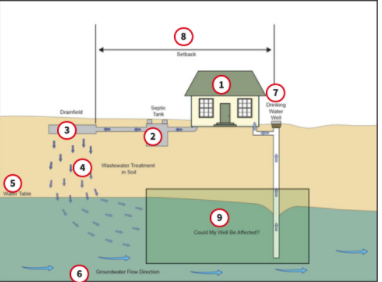
\includegraphics{images/Circular-Images/septictank_image.png}
\caption{Illustration of a septic tank}
\label{fig:Septic Tank}
\end{figure}

Septic systems are a linear form of disposal as they release high concentrations of methane (CH4) into the atmosphere. Methane is 30 times more powerful than CO2 and comprises 16\% of global GHG emissions \citep{fu_schleifer_zhong_2017}. A study found 85\% of households in Hanoi, Vietnam; Mandalay, Myanmar; and Kota Surakarta, Indonesia use septic systems \citep{huynh}. While many use different designs, it was found they all release methane CH4 through anaerobic decomposition. The United States Environmental Protection Agency (USEPA) estimated global methane production from septic systems as 3.0 Tg-CH4 per year, which is 10.4\% of global CH4 emissions from domestic wastewater \citep{e_p_a}. Because of the study, CH4 emissions from septic tanks are now roughly accounted for in net global GHG emissions. Many septic systems in East Asia do not have a drainfield, they process only sewage, while sullage is emptied into the environment. The climate of Southeast Asia (77-97°F) promotes anaerobic digestion conditions increasing GHG emissions \citep{huynh}. The study found high concentrations of CH4, CO2, and dismissal amounts of N2O in septic tanks in Hanoi. The table below illustrates CH4 emissions reflective of the amount of time sewage remained in septic tanks. The study found if septic tanks are regularly emptied, there are less GHG emissions.

Figure \ref{fig:Methane}
\begin{figure}
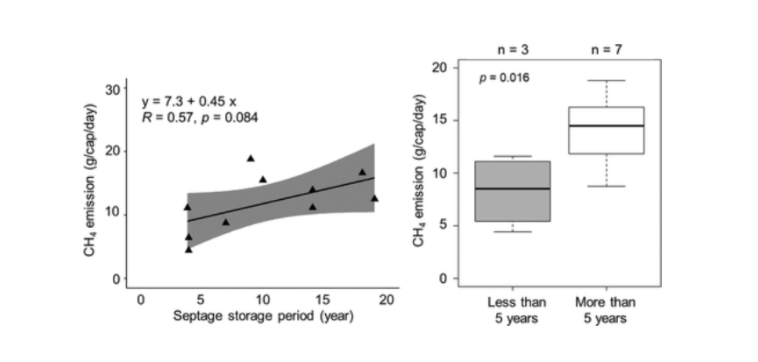
\includegraphics{images/Circular-Images/Methane_levels.png}
\caption{Illustrates CH4 levels in septic storage over periods of time}
\label{fig:Methane}
\end{figure}


The CH4 found in the average septic tank in Hanoi was oversaturated by 24,444\%, while the CH4 in lagoons when measured was 260–128,420\% \citep{huynh}. Therefore, when compounded, septic tanks in Hanoi, and other parts of SE Asia, contribute greatly to atmospheric methane levels. Additionally, sewage was reported to be released into a non centralized sewer or directly into a waterbody, demonstrating the linearity of present septic systems in Hanoi and much of SE Asia. The study shows only 2-6\% of sewage in Hanoi was treated at a sewage facility, some went to a landfill site, and unknown amounts were disposed of illegally \citep{huynh}. The study found the average septic tank to have CH4: 11.92 ± 4.52 g/capacity/day, while CO2 was 20.24 ± 9.15 g/cap/day. Septic tanks are effective at reducing pathogens, however, their methods of disposal are linear as they do not not capture or resource CH4 for energy, thus they release methane, a very potent GHG into the environment. They also, often, do not resource nitrogen and phosphorus for fertilizer. Additionally, if chemicals are present in the effluent, they are released into the groundwater \citep{huynh}. 

\subsection{Vietnam’s Double-Vault Latrine: A Circular Treatment Comparison To Septic Systems }

For centuries farmers in Vietnam and China used untreated human excreta and urine as a fertiliser for rice and other crops (nitrogen in excreta and phosphorus in urine, are extremely rich materials for fertilizer). However, in 1956, to combat the hazardous practice, Vietnam health authorities instituted the first double-vault composting latrine program, which uses similar principles, but with sanitary measures \citep{pebler}. Since then DVC technology has been widely supported and adopted by other countries. In 2007 the Government of Vietnam assessed 25\% of rural households were without a toilet (to be further referred to as a latrine), and 19\% were found to have an unhygienic latrine \citep{cole_phuc_collett_2009}
. Given the startling figures, Vietnam implemented a goal of constructing 2,600,000 hygienic latrines by 2010 \citep{cole_phuc_collett_2009}. The government compared the double-vault composting latrine (DVC latrine), the septic tank latrine, pour-flush water sealed latrine and ventilated pit latrines, and found the most hygienic, as well as versatile, system to be the DVC latrine, which the Government subsequently funded.

The DVC latrine is simple, easily constructed, requires moderate maintenance, is cost-effective(\$70 us), and creates a valuable byproduct. The DVC is a closed-cycle-system: it saves water, prevents groundwater pollution, and produces a fertilizer/soil conditioner for agriculture. Treated human excreta can be used as a fertilizer to increase the water holding and ion-buffering capacity of soil \citep{cole_phuc_collett_2009}. Proper construction and use of the DVC are important, so as to prevent pathogenic contamination on agricultural produce. 

How it works: The DVC can be built above or in the ground, if in the ground, the water table should not be close. The DVC consists of two vaults, one is in use, the other contains decomposing excreta. Each vault is ideally built two accommodate one year of excreta. Excreta enters the vault free from urine (it is a dry system and urine is collected in jars). Sawdust or ash are thrown into the vault after each use, reducing moisture content. When the vault is 75\% full, it is completely filled with dry Earth and the squat hole is sealed. For the following 6-12 months microorganisms (aerobic and anaerobic) decompose the excreta and pathogens die (the vault is often painted black to increase the rate of dehydration, and solar panels can be used) \citep{nzdl}. During this time the other vault is used. After said time, the decomposing vault is emptied and used for fertilizer. Figure \ref{fig:DVC Latrine}


\begin{figure}
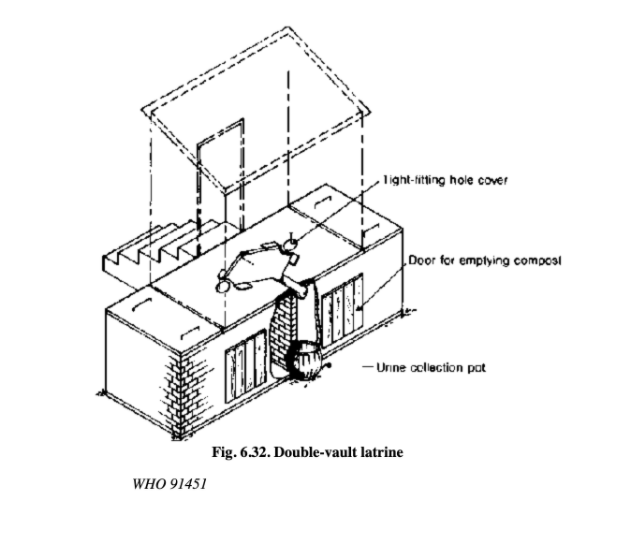
\includegraphics{images/Circular-Images/DVC_image.png}
\caption{Representation of the DVC Latrine}
\label{fig:DVC Latrine}
\end{figure}

A study found that after emptying decomposed containers, 63\% of households immediately used the contents for fertilizer; the remaining households conducted a secondary form of composting. 61\% of households reported using urine on crops and garden trees. Researchers found 91\% of households were satisfied with the DVC latrine. However, 73\% of households reported emptying the vault 1-2 times per year, prior to rice planting (February and June). This suggests the vaults were often emptied before the recommended 6-12 month storage period \citep{cole_phuc_collett_2009}. Reported problems with the system were fly pestilence and odors. Ultimately, the DVC is a more circular system than the septic latrine as it produces fertilizer and preserves water; nonetheless, it still releases GHGs. 

\subsection{Municipal Utility Sewage Treatment: Linear}

Many parts of SE Asia do not have the funds for large scale wastewater treatment facilities like those present in Europe and the United States. Although developed countries have formidable facilities, the majority use linear processes that refine water (as described by aerated septic systems) but do not capture GHGs produced through anaerobic microbial decomposition. Sludge waste collected through water refinement, is sent to landfills where CH4 and other GHGs are furthermore released \citep{usgs} \citep{epa_2018}. 

\subsection{The Anaerobic Digester and Biogas: Circular Sewage Treatment}

According to the United Nations, 80\% of wastewater flows into the ecosystem without being treated or reused. This creates a multitude of problems for the environment and human health: great amounts of GHGs are released into the atmosphere and roughly 1.8 billion people drink and use the pathogenic water, risking infection: cholera, dysentery, typhoid and polio, and ingest of toxic chemicals \citep{u-n}. 

Polluted rivers contribute significantly to global warming. The New Territories of Hong Kong may appear clean and lush with agricultural fields, expansive greenery and mountains; however, in reality, the rivers flowing through these areas are saturated with three primary greenhouse gases: methane, carbon dioxide, and nitrous oxide. A study found the concentration of said gases were 4.5 times greater in the rivers flowing near Hong Kong, than found at atmospheric levels. The cause of pollution is discharge from agricultural livestock (farm waste contributes to 58\% of world methane emissions) and human effluents \citep{smith}. “It's estimated that rivers and streams release up to 3.9 billion tonnes of carbon each year (around four times the amount of carbon emitted annually by the global aviation industry)\citep{bbc_news_2019}. Moreover, it’s estimated global rivers and lakes are the cause of more than 50\% of atmospheric methane concentrations, largely due to unrecovered methane in untreated wastewater. The more polluted the rivers, the higher the emissions. ``When rivers become polluted, their global warming potential (GWP) can increase from two to 10 times'' says Long Tuan Ho, researcher at Ghent University, Belgium \citep{matthew}. Moreover, the CO2 and N2O concentrations of water zones close to urban areas were found to be four times higher than those at natural sites; in the case of methane, this ratio was 25 times higher. Again, the primary culprit is untreated wastewater runoff. When untreated effluents enter bodies of water, biogeochemical reactions occur via anaerobic microorganisms which create GHGs (CO2, N2O, CH4), consequently resulting in a positive (warming) feedback loop. The septic system, double-vault-composting latrine, and the vast majority of municipal wastewater treatment sites release GHGs into the atmosphere. These linear waste management systems are increasing the rate of global warming and untreated wastewater is infecting limited drinking water supply with pathogens. 

Water is precious and so is energy. Anaerobic wastewater digestion with biogas recovery is a circular “waste-to-energy technology” that can greatly reduce world methane emission, furthermore, the captured CH4 can be used for a variety of human energy needs. The system is low-cost, readily available, carbon-neutral, and reduces environmental degradation caused by fossil fuels. 

How it works: During natural decomposition, anaerobic microorganisms transform biomass (organic matter—sewage, food waste, animal manure) into methane gas and digestate (the material that remains after anaerobic digestion). Biogas can be converted into electricity or fuel, and then used throughout the energy sector, ie: cooking, lighting, transportation, building conditioning \citep{wilkie}. Digestate is nutrient dense and can be used as a non synthetic fertilizer for crops. Biogas is 40\%–60\% methane, the remainder is CO2, small amounts of water vapor, and other gases. Biogas can be burned directly, used to generate electricity, or treated to become biomethane--a low carbon “pipeline-quality” fuel \citep{eia} \citep{environmental_and_energy_study_institute_(eesi)} \citep{epa_2018} \citep{wilkie}.

When methane is burned, the potent GHG is transformed into energy and CO2 is released. While CO2 is also a potent GHG, the CO2 being produced is not adding new carbon to the atmosphere, this is the CO2 naturally sequestered by plants––thus the CO2 is carbon neutral. Burning methane is far better than having it escape into the atmosphere. If biogas is used in place of fossil fuels, the net emissions are “negligible” in comparison \citep{fu_schleifer_zhong_2017}. While many wastewater treatment centers have anaerobic digesters, the majority do not have energy recovery systems, thus they incinerate sludge or dispose it into landfills, which releases methane, CO2 and nitrous oxide into the atmosphere; consequently, these linear disposal systems increase the rate of climate change and society loses a valuable source of energy. Wastewater treatment with biogas-recovery systems are an example of circular waste management: they save money, capture energy, and reduce global warming.

A pilot project in Xiangyang, China, illustrates how sludge to energy refinement can power the treatment facility itself, recover valuable nutrients and energy, reduce GHG emissions, prevent land and water pollution, and be cost-effective. Over the course of its lifetime, the treatment facility reduces GHG emissions by more than 95 percent \citep{liu}. A 2015 report found the plant can supply 300 cars with natural gas daily. The system is also profitable making the plant \$ 1.5 million annually. Four large cities in China: Beijing, Changsha, Chengdu and Hefei have implemented, or plan to install, sludge to energy facilities, which will reduce 700,000 tons of CO2 emitted per year and are estimated to produce 40 millions cubic meters of compressed gas to be used by municipal vehicles \citep{wri_2015}.  

Developing countries lacking sewage treatment infrastructure can benefit greatly at the village and city level by adopting sludge to energy systems. This is exemplified at the local level in Indonesia as 80\% of Indonesian households dispose their waste into septic tanks; 60\% of these septic tanks are located less than 32 feet from the household wells which results in high concentrations of E. coli in drinking water \citep{andriani2015review,}. Similar conditions are described in Vietnam and other SE Asian countries. \href{https://www.youtube.com/watch?v=9kKRdlAFuZw}{Small and affordable} (\$ 35-100 usd) decentralized digesters can be used at homes for kitchen waste as well as for livestock and human excreta \citep{worldbank}. The biogas produced can be used directly for cooking and electricity generation. Educating and supporting low-income communities to use anaerobic digester systems will reduce deforestation for firewood, improve water quality, and mitigate climate change. Further research may elucidate if anaerobic digesters can be used in conjunction with the double-vault-compost latrine and septic tanks. 

Biomass to energy systems can be applied to any form of organic waste; therefore, 3.9 trillion kg of human/livestock faeces p/y and the 1.3 billion tonnes of global food wasted each year, could be repurposed and turned into carbon-neutral energy \citep{fao}. The electricity generated from biogas could meet the needs of about 40 million people globally, 22 percent of global electricity consumption” \citep{aquatech}. By 2030 it is estimated the planet will be generating more than one trillion kg of faeces each year, this number is expected only to rise with population growth \citep{berendes_yang_lai_hu_brown_2018} \citep{un}. The rising population with associated life consumption waste (food, agriculture, and excreta), makes biogas sequestration a great circular and sustainable technology for wastewater treatment. According to Niclas Svenningsen, manager for the Global Climate Action team at the United Nations:

``[Biogas] is a win-win-win-win-win industry: win for turning GHG into energy; win by using that energy to replace fossil fuels; win by turning global waste, that releases dangerous levels of methane gas every day, into a valuable resource; win by creating jobs and contributing to the new low-carbon economy; win by offering a stable energy source that can be built and used even at the household scale in remote areas'' \citep{hughes_2019}.
Biogas is a highly recommended wastewater-nutrient-energy technology for the world and SE Asia.

\subsection{Phytoremediation: Wastewater Circularity}

Phytoremediation, ``plant remedy,'' is considered an effective, aesthetically pleasing, and cost-effective sustainable wastewater treatment technology which is governed by the principles of interdependence and circularity \citep{ali2020application}. Phytoremediation has been used for the last 300 years, but became well known in 1983 \citep{stephenson2014one}. A phytoremediation site can treat a multitude of industrial and municipal pollutants including: pesticides, chlorinated solvents, polycyclic aromatic hydrocarbons (PAHs), Polychlorinated biphenyl (PCBs), petroleum hydrocarbons, radio nucleosides, surfactants, explosive elements, heavy metals\footnote{ Heavy metals are said to cause damage to DNA and produce carcinogenic effects in animals and humans \citep{kaur2020role}. Linear waste activities such as mining, municipal waste, application of fertilizer, discharge of urban effluent, vehicle exhausts, waste incineration, fuel production, and smelting release heavy metal contaminants into the wastewater stream (1).}, as well as sewage and livestock excreta. Phytoremediation prevents soil erosion reducing the spread of contaminants (groundwater leaching can occur) \citep{ali2020application}. The treatment method is cost-effective, and does not require exclusive equipment or highly trained workers. The clean up cost is dismal, giving it a special place among green technologies. The disadvantages include a slower treatment time, possible source of dangerous mosquitoes, and is limited to shallow contaminants \citep{mustafa2020recent}. The aquatic plants (macrophytes) used have the following characteristics: they are fast growing, produce a high biomass yield, transport metals and pollutants into above ground part of the plants, and can tolerate high levels of metal toxicity. 

Plant selection is the most important aspect of phytoremediation. Water hyacinth (Eichhornia crassipes), water lettuce (Pistia stratiotes) and Duckweed (Lemna minor) are prominent phytoremediation plants. These plants create a thriving environment for microorganisms, fungi and bacteria, providing them with enzymes from their roots. The microbes reduce pathogens and metal toxicity; they also provide plants with nutrients, increasing a plant’s phytoremediation ability \citep{kaur2020role}. This plant-microbe mutualism showcases circularity in action. Figure \ref{fig:Phytoremediation Facility and System}

\begin{figure}
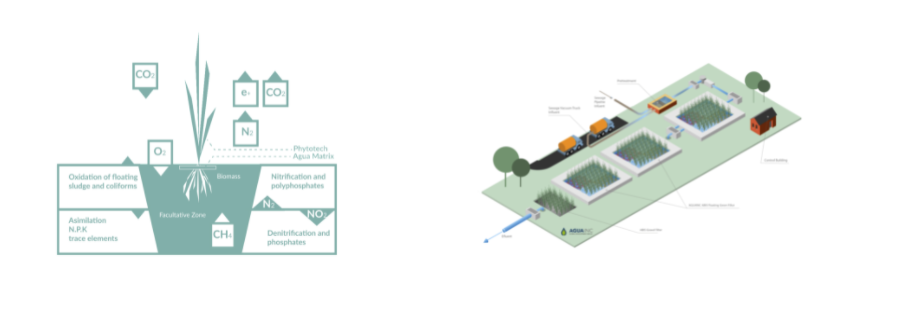
\includegraphics{images/Circular-Images/phytoremediation.png}
\caption{Phytoremediation facility and how the biotechnology works}
\label{fig:Phytoremediation Facility and System}
\end{figure}

How phytoremediation works: Wastewater travels through matrices of floating plants, the plant’s roots filter the water (rhizofiltration), absorbing nutrients and heavy metals. The leaves above water sequester carbon and hold pollutants. During photosynthesis, the plants release oxygen, aerating the water for aerobic microbes, which in turn break down faecal pathogens and supply nutrients to plants. 

Water hyacinth (Eichhornia crassipes) has been deemed a problematic and invasive plant because of its high growth rate, but is now used for phytoremediation technology. Water hyacinth is the recommended treatment plant for industrial wastewater, domestic wastewater, sewage effluents, and sludge ponds because it absorbs high rates of organic and inorganic contaminants, can tolerate extreme pollution, has a high biomass production rate, absorbs nitrogen and phosphorous, and can remediate metals like arsenic, zinc, mercury, nickel, copper and lead \citep{mustafa2020recent}. The associated wastewater processing time of water hyacinth is 1-2 months \citep{mustafa2020recent}. Sewage pathogens are broken down by predators, protozoa and bacteriophages, living near the plant’s roots \citep{aguainc_2015}. Nitrogen, a rich element present in sludge, leads to the eutrophication of the environment, while phosphorus (present in urine) can lead to cyanobacterial (algae) blooms causing ecological imbalances \citep{aguainc_2015}. Nitrogen and phosphorus accumulate in the roots of water hyacinth, which can be later harvested for compost, fertilizer, and biofuel \citep{kulkari} \citep{aguainc_2015}. Metals that have accumulated in the plant stem and leaves can also be recovered \citep{aguainc_2015}. Phytoremediation plants can be used in all forms of wastewater treatment, as well as implemented in rivers and other bodies of water. Phytoremediation is an important circular technology, treating a variety of pollutants. It is a sustainable bio-wastewater treatment system that can provide solutions to communities through SE Asia and other parts of the world. 


\begin{figure}
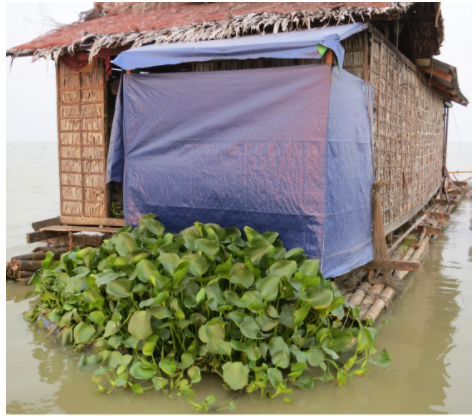
\includegraphics{images/Circular-Images/HandyPod_image.png}
\caption{The HandyPod}
\label{fig:HandyPod}
\end{figure}

In Cambodia, about 100,000 people live in floating communities on the Tonle Sap Lake \citep{wetlands_2019}. During the low-water dry-season, much of the community's ambient water becomes infected with human excreta. Children, especially, are at high risk of pathogenic exposure as they play in the lake’s water. Wetlands Work, a social enterprise, has developed the “Handy Pod,” a circular, cost-effective, waste water treatment system for these floating communities (Figure \ref{fig:HandyPod}). The system uses microbes and phytoremediation to refine sewage to “grey water” levels––deemed low risk. The effluent quality tested 28-100 colony forming units (cfu)/100 ml in a one-half cubic meter volume of ambient water; this is significantly less than the Cambodian standard maximum: 1000 cfu/100 for contact recreation water quality. The system reduces E-coli by \href{https://www.youtube.com/watch?v=VmRO6nPIIc8&t=2s}{99.9\%}.

The Handy Pod costs \$ 30US  to assemble. It is then placed beneath the floating house’s latrine. After use, excreta travels into an expandable bag, which is treated by naturally occurring microbes, the remaining effluent is then processed by water hyacinth plants, pathogens stick to their roots and are further broken down by microbes. The treated water then flows into the lake \citep{akpan_2014}. The Pod was tested for three years and has been deemed successful. It has no smells, is aesthetic, there are no mosquitoes, no chemicals, it has demonstrated stability during storms, and requires little to zero maintenance. While problems still face the Handy Pod, like residual pathogens, it is a positive step forward for sanitation in impoverished zones. It illustrates how small circular systems can be made, as well as exemplifying the effectiveness of microbial digestion and phytoremediation. A point of further research is to know if biogas recovery systems could be implemented in conjunction with the Handy Pod.

\section{Linear Chemicals in Wastewater: Pesticides in Taiwan}

Pesticides and chemicals are a concern for wastewater treatment since they pass untreated through the majority of wastewater facilities, collecting in humans, animals, and the environment. Synthetically formulated pesticides became widespread after WWII. They enable large farm yields; nevertheless, pesticides are toxic to humans, animals, and a large number of non-invasive insects. Many pesticides are “persistent” (not breaking down easily) so they don’t have to be reapplied often, and they are hydrophobic, to not be washed off by rain. Pesticides are a classic example of a linear product that is low cost, used widely, results in great yields, and is of  harm to humans and the environment \citep{oregonstate}. Today synthetic pesticides are still used throughout the world, especially in SouthEast Asia where agriculture is a principal commodity. 

Taiwan is a relatively small island in SE Asia (13,974 mi$^2$), surrounded in the north by the East China Sea and to the south by the Pacific Ocean. Located in the semi-tropics, Taiwan is one of the most densely populated islands in the world with 23.57 million people 
\citep{bbc_news_2019}. 
The following case study examines the presence of toxic pesticides located in the Danshui River (largest river in Taiwan), which ultimately passes through a waste treatment plant; pesticides still flow into the ocean. Figure \ref{fig:Danshui River Pesticides} illustrates points of sampled sediments, the greatest being at D13, the wastewater treatment site.

The island experiences a dry and wet season. During the dry season, pesticides were found in river sediments. During the wet season, characterized by winter and summer/fall monsoons, pesticides were found in the ocean ecosystem and marine organisms. The river is defined as a primary transport process and the ocean as a second transport process. Each section of the river is important and sheds light on understanding the pesticide life-cycle in the environment. The Da-han River (top of the Dan Shui) brings fresh water to agriculturists; the Shin-dan River (mid-point of the Dan Shui) provides water to tea farms in drinking water for citizens in Taipei (2.646 million inhabitants) and neighboring counties; finally, the Keelung River (last leg of the Dan Shui) is distinguished by many industrial plants located within the the river’s drainage basin; The waste-water treatment facility located at the mouth of the estuary (where the river flows into the ocean) was the point of highest pesticide contamination and is where oysters and other sea creatures were found to have pesticides in their bodies \citep{hung2007relationships}. 

\begin{figure}
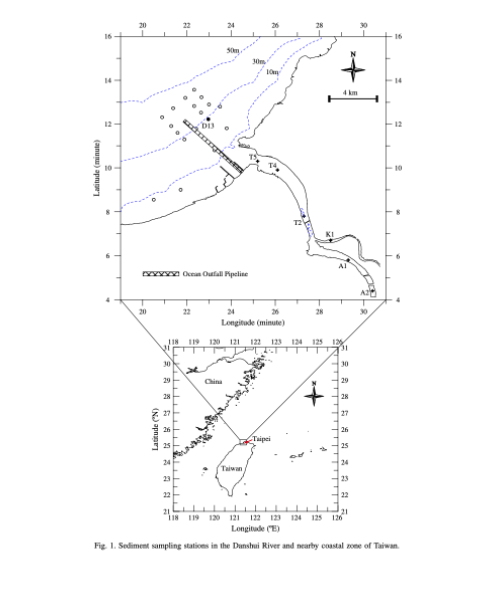
\includegraphics{images/Circular-Images/Danshui_image.png}
\caption{A representation of the advantages of a Circular Economy}
\label{fig:Danshui River Pesticides}
\end{figure}

The pesticides were found in sediments and the marine ecosystem. Pesticides, which are made from hydrophobic carbon-chain molecules, adhere to carbon-based particles in the water, which eventually fall into river sediments. The pesticides are “sticky” and layer onto each other. There are many pesticides in use (tetrachlorobenzene, HCHs, aldrin, dieldrin, chlorpyrifos, mirex, DDEs, DDDs, and DDTs) and it becomes hard for scientists to differentiate between them since they mesh together \citep{hung2007relationships}. When the chemicals enter the marine ecosystem they attach to phyto-plankton which are ingested by clams and fish, which die and enter ocean sediments or are consumed by other aquatic organisms, or humans (Huertos, conversation). 
``The sum of pesticides, including tetrachlorobenzene, HCHs, aldrin, dieldrin, chlorpyrifos, mirex, DDEs, DDDs, and DDTs, was found in offshore sediments at station D13, approximately 6e7 km from the Danshui River mouth (Fig. 1). Coincidently, the discharge point, with several output pipelines connecting to the main pipeline, of the marine outfall pipeline from the Pali sewage treatment plant is located near this station (Sinotech, 1997)...... Therefore, the fact that individual pesticide concentrations that are found at the station near the marine outfall pipe are high or highest suggests that the sewage treatment plant is still discharging pesticides from residual activated sludges and/or fine particles'' \citep{hung2007relationships}.
Pesticides from present and past agricultural practices were found in the ecosystem, illustrating pesticide persistence. This study illustrates the importance of understanding where pesticides end up (always into the ecosystem and into organisms) and their main outlet source. The Pali sewage treatment plant illustrates how many municipal wastewater treatment facilities ineffectively treat pesticides. Pesticides are illustrated here as single-use linear products, which pass through waste management systems, accumulating in the environment and harming organisms. This is of great concern as pesticides exposure has been linked with health defects in humans, animals, and plants \citep{sharma2019responses}. This study also raises questions on the quality of drinking water in Taipei. 

\subsection{Pesticides in Taipei Food Toxicology: (further research is needed for drinking water)}

Taiwan ranks third globally in pesticide usage “per unit of area planted” (Japan is number one). Without pesticides, the annual output of rice would decrease by 15\% the first harvest and 30\% the second (similar results would occur with other produce) \citep{ministry_of_foreign_affairs}. Nonetheless, pesticides are problematic for the environment and detrimental to human and animal health. Acute exposure to humans can cause: stinging eyes, rashes, blisters, blindness, nausea, dizziness, diarrhea and death. Known chronic exposure can result in: cancer, birth defects, reproductive harm, neurological and developmental toxicity, immunotoxicity, and disruption of the endocrine system \citep{nicolopoulou2016chemical}.  
Pesticide awareness is growing and many people throughout SE Asia are raising the red flag. Greenpeace, an NGO in Taiwan, measured pesticide residue on 60 vegetables and fruit sold at major retail outlets throughout Taiwan: RT-Mart, Pxmart, Carrefour, Wellcome, A. Mart, Costco, 7-Eleven and FamilyMart. The study found 73\% (44/60) of the tested specimens contained pesticide residue, 27\% (12/44) were above pesticide safety levels, and five contained prohibited pesticides \citep{ministry_of_foreign_affairs}. These dangerous chemicals were found in oranges and passion fruit from A. Mart, as well as oilseed, lettuce and jujubes from Carrefour. Green beans from Costco were found to contain fungicide residue 69 times higher than the legal amount. Lo Ko-jung, the project manager at Greenpeace said: 
``The solution to pesticide residue in food relies on retailers proposing specific measures to ban pesticide-containing products, but Costco ignores the consumer’s right to know because it has refused to disclose its pesticide management policy'' \citep{ministry_of_foreign_affairs}.
Trade secrecy laws allow manufacturers to exclude specific ingredients or chemical quantities on labels if doing so would decrease profit—illustrated by Costco. 

Pesticides are a waste management issue because agriculture runoff and improper disposal release pesticides into wastewater flow, processed by treatment facilities lacking expensive pesticide removal technology; consequently, pesticides enter humans and the environment. If dangerous substances are passed untreated through wastewater treatment facilities, they are a waste management issue—this is regarded to be true for any synthetic chemical. Most countries in SE Asia lack a pesticide waste management framework, 80\% of pesticides are imported illegally and are uncontrolled, they are cheap and high in toxicity \citep{thuy2012current}. Pesticides are a linear commodity whose end-life produces toxic water, which accumulates in sediment, enters living organisms, or circulates through the hydrologic cycle \citep{thuy2012current}. Pesticides and other chemicals are regarded here as neither technical nor biological nutrients, as they pose a threat to humans and the environment alike. 

\subsection{Circular Biopesticides: An Alternative To Hazardous Synthetic Pesticides}

A circular alternative to pesticides are biopesticides and bioherbicides. They have been used since the 1950’s but are now gaining global attention as they provide a sustainable and safe alternative for agricultural needs stefanski2020potential \citep{hubbard2014biochemistry}. Biocontrol products are produced from naturally occuring funguses, microbes, plant metabolites, and biochemicals, which mitigate unwanted pests and weeds with little or no health/environmental effects. “Biopesticides from fungi are employed to control weeds, beneficial bacterial pesticides are used to control fungal and bacterial disease and viral pesticides are used to resist insect pests” \citep{usta2013microorganisms}. The most effective biopesticides have been reported to be those which utilize compounds produced by microorganisms. Chemicals created by microbes produce toxic proteins, their production can be optimized through fermentation. Biopesticides target pests and do not negatively impact human health, animals or the environment, they are therefore circular and can be regarded as effective alternatives compared with synthetic pesticides. 

Their advantages and disadvantages include the following: biopesticides are not “persistent,” they break down into the environment becoming part of the biosphere, thus creating a closed cycle. Because of their short life, more biopesticide application is required, this can potentially boost job markets. Bioinsecticides do not cause air or water quality problems. They often contain Bacillus thuringeinsis, a microbe which targets specific pests without harming other beneficial organisms (pollinators, humans, animals, etc). Nevertheless, if many pests are present, selective methods do not serve the intended purpose of a pesticide (however, given biopesticides come in multiple forms, this caveat may be remediated) \citep{mccoy2020organic}. The creation and application of biopesticides is often more complicated and their use requires more knowledge, for instance, nematodes must be refrigerated and used within two weeks for effectiveness. Thus, education is important for biopesticide implementation. Furthermore, biopesticide microbes utilize “multiple modes of action” preventing pest resistance; this is advantageous as synthetic pesticides use “single modes of action,” which pests become resistant to \citep{hubbard2014biochemistry}. While initially more expensive, natural pesticides do not cause health issues, thus saving one from suffering and health expenses in the long run. Additionally, biopesticides have a registration time of less than a year (because they are seen as less dangerous), compared with synthetics which call for three years \citep{mordor}.

More than 225 microbial biopesticides are currently being manufactured in 30 countries in the Organization of Economic Development and Cooperation. The US, Canada, and Mexico account for 45\% of all biopesticides sold; Asia accounts only for 6\% which demonstrates Asia’s lack of organic agriculture practice, yet presents an incredible opportunity for SE Asia to increase its health/environmental wellbeing, while also increasing economic prosperity \citep{hubbard2014biochemistry} \citep{mordor}. A shift in pesticide use is now occurring in Asia as countries like Vietnam are recognizing the advantages of using bioinsecticides. The biopesticide market is expected to reach USD 60.61 million by 2024 \citep{marketwatch_2021}. The International Rice Research Institute (IRRI) has called for a ban of certain synthetic pesticides, increasing awareness and demand for biopesticides in SE Asia. China was recently placed first in the field of biopesticides research and development worldwide \citep{mordor}. Demand for sustainable agriculture is building and biopesticides are an important part of the shift. Further research in biotechnology and chemistry can potentially help lower biopesticide prices and increase their presence throughout the world, especially in SE Asia \citep{hubbard2014biochemistry}.

\section{Further Research Needed: Linear Chemical Waste一``Forever Chemicals''}

An individual chemical can persist in the environment for long periods of time, moreover, they build up. The majority of these man made chemicals are polyfluoroalkyl substances (PFAS: PFOAs and PFOs) (different from pesticides): they are a broad class of more than 5,000 chemicals used in a great number of products including “clothing, furniture, nonstick cookware, food packaging, firefighting foams, and electrical wire insulation,” furthermore, they are found in seafood, agriculture produce, and drinking water \citep{hersher_2019}. Linda Birnbaum, the director of the National Institute of Environmental Health Sciences and the National Toxicology Program, says: ``We're finding them not only in the environment, but we're finding them in people'' \citep{hersher_2019}. These persistent materials are called “forever chemicals,” and are resilient to natural degradation processes––chemical, biological and photolytic––because of strong covalent bonds between carbon and fluorine atoms \citep{acs}. PFAS can dissolve in water, and because of their chemical properties, traditional wastewater treatment technologies are not able to remove them \citep{epa_2018} \citep{ipen}. These chemicals often enter into organisms through water or food, bioaccumulating in tissues and binding to proteins; as organisms are consumed, the chemicals cycle through the food chain, just like pesticides. In humans PFAS are often found in blood, liver and kidneys \citep{ipen}. However, recent studies have found PFAS contamination in breast milk in India, Indonesia, Japan, Sri Lanka (bood), Malaysia, and Vietnam which have been found in fetus’ \citep{ipen}.

Epidemiologists have found a ``probable link'' between long-term exposure to the PFAS chemicals and certain medical conditions such as: kidney cancer, thyroid disease, (female and male) infertility and developmental effects, lung defects, and more. These chemicals are also found in the blood, liver and kidneys of wildlife. Sewage treatment plants have been identified as major polluting sources of PFAS, evidenced by Japan, Thailand, Vietnam and other countries \citep{ipen}. These chemicals are linear, and circular solutions are deemed necessary to phase them out internationally \citep{land2018effect}. 

There are many valuable resources present in wastewater; however, these do not include pesticides and “forever chemicals.” It has been 82 years since industrial chemicals (PFAS and pesticides) were first created, yet they are still causing harm to humans and the environment, and still people don't know what to do with them. Phasing them out and replacing them with alternatives is a priority.

\subsection{Household Products}

The average home throughout the developed world contains a multitude of cleaning products which may contain forever chemicals. Given cleaning products’ wide usage, they are often overlooked as dangerous to human and environmental health. When cleaners are washed down the drain by millions of people, even trace amounts become a serious problem. The problem extends to septic tanks and municipal sewage \citep{bown}. 

Municipal sludge, a valuable fertilizer, often cannot be repurposed because it’s laden with pharmaceuticals, chemicals and PFAS, which make people and the environment sick through fertilizer use \citep{perkins_2019}. Global wastewater can contain hormones, pathogens, heavy metals (lead, cadmium, arsenic and mercury), as well as chemicals: pesticides, pharmaceuticals, PCBs, PFAS, BPAs and other harmful substances \citep{perkins_2019}.  Effective wastewater treatment addresses the conglomerate of elements present in water. Given wastewater treatment plants in developed nations still emit dangerous chemicals, their expensive installation is not an advisable trajectory for developing nations to follow, rather a global phasing out of “persistent” toxic substances is in order. Further research is needed to understand PFAS wastewater treatment and how to phase them out. 

\section{Conclusion}

The linear production model will not sustain life on Earth. Consumption is a necessity for life, but creating waste is not. Energy, which constitutes all things, can neither be created nor destroyed, it only changes form. It makes sense for humans to live in accordance with this law of the universe; circular systems are a way to do so. Circular economics is being pushed forward as a new alternative, nevertheless circular living has been iterated for thousands of years by first nation people, who to this day live in this way. Through biomimetic systems, society can exist in synergy with the environment. The circular economy is underdevelopment and has a ways to go, but as illustrated by case studies from SE Asia, bio-regenerative-wastewater-treatment-systems with ingredient recovery are fundamental to its realization. 

The double-vault-compost latrine, the anaerobic digester, and phytoremediation use natural microbes to treat wastewater, thus demonstrating how humans can design with nature's existing systems. Valuable nutrients: fertilizer, bioenergy, and metal, can all be recovered through engineered solutions informed by natural chemistry. Similarly, by understanding microorganisms, biopesticides are developed. These case studies demonstrate SE Asia and the world can benefit greatly by adopting bio-regenerative-wastewater-treatment-systems, increasing wellbeing, environmental protection, and economic prosperity.Figure \ref{fig:Circularity} 

Further research is needed to understand how to remediate PFAS and other toxic chemicals including pharmaceuticals and cleaners; to understand the low-cost construction details of decentralized anaerobic digesters and how they can be attached to DVC latrines, and septic tanks (Gihiandelli, 1; Mang, 1). Questions to be further researched: what circular biomimic innovations can be made for landfills; how can further research into interconnectivity resolve societies issues; how can existing linear systems and supply-chains be made circular? 


\begin{figure}
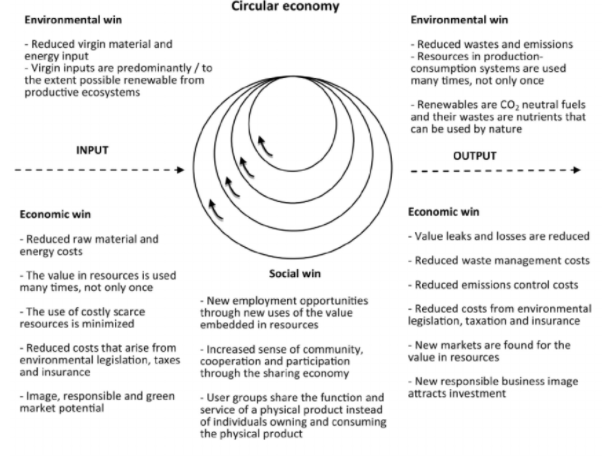
\includegraphics{images/Circular-Images/CircularEconomy_image.png}
\caption{A representation of the advantages of a Circular Economy}
\label{fig:Circularity}
\end{figure}




\chapter{Plastic and Packaging in Japan}

\section{Introductiona and Goals?}

Plan: Use Japan's unique plastic packaging as a lens to view plastic waste management. I can bring in benefits of their plastic use, like cultural significance of beautiful wrapping and food safety, and then discuss plastic pollution as a larger issue in East Asia, bringing in examples of blame placing, and of course discussing potential solutions on both international and local scales. 

\section{Plastic Pollution and Waste Management in East Asia} 

\subsection{Statistics/comparisons}

graphs and images will help with perspective

\subsection{History of plastic waste issues in East Asia}

\subsubsection{Are specific companies/industries responsible responsible}

what kinds of plastic waste are there (sector break down)? 

\subsubsection{Where in the world did the ubiquitous usage of single use plastics come from?}

General blame placing/biases/rhetorical 

examples of discourse around plastic waste in East Asia. Why does any of this matter(needs its own section)?

Plastic waste trade? 

\url{https://link.springer.com/article/10.1007%2Fs10163-004-0115-0}

\url{https://www.sciencedirect.com/science/article/abs/pii/S0956053X20305602}

Blame placing through both rhetoric and scientific studies

(this source is a very data based study that concluded that the vast majority of plastic pollution comes from a few sources in Asia/Africa... I want to explore what they might not have taken into account when collecting data)

\url{https://science.sciencemag.org/content/347/6223/768}

\url{https://pubs.acs.org/doi/10.1021/acs.est.7b02368}

\url{https://www.dw.com/en/whose-fault-is-plastic-waste-in-the-ocean/a-49745660} (found the two above studies through this article)

Japan Specific (I need to break these into hierarchies of significance), some sections, the first  few will be more data based, the second half will be more rooted in sociological primary sources.

Waste management issue overview

Sector Break Down/ responsible parties in Japan

Impacts of plastic pollution on different groups within Japan

Cultural significance of wrapping

Food safety

Gov action/recycling/current efforts

Activism

Potential solutions moving forward rooted in current activist efforts/respect to culture

\url{https://www.pnas.org/content/117/33/19844.short}

\url{https://www.jstor.org/stable/432317?seq=1}

\url{https://onlinelibrary.wiley.com/doi/abs/10.1002/1099-1522(200003/04)13:2%3C45::AID-PTS496%3E3.0.CO;2-%23}






\backmatter

\part{Backmatter}

The back matter often includes one or more of an index, an afterword, acknowledgments, a bibliography, a colophon, or any other similar item. In the back matter, chapters do not produce a chapter number, but they are entered in the table of contents. If you are not using anything in the back matter, you can delete the back matter TeX field and everything that follows it.

\printglossary

\renewcommand\bibname{References}
\setlength{\bibsep}{2\baselineskip}
\setlength\bibindent{.5in}
\bibliographystyle{plainnat}
\bibliography{References}

\end{document}
